\documentclass{article}
\usepackage{amsmath, amssymb}
\usepackage{braket}
\usepackage{graphicx}
\usepackage{vcounter}
\usepackage{hyperref}

\begin{document}

\newcommand{\A}{\ensuremath{\mathbb{A}}}
\newcommand{\I}{\ensuremath{\mathbb{I}}}
\newcommand{\M}{\ensuremath{\mathbb{M}}}
\newcommand{\AIM}{\A\I\M~}


\title{\AIM Semantics for Causal Procedures}
\author{Julia Turcotti, v0.0.\vcounter}
\maketitle

\tableofcontents

\section{Preliminaries}

This document outlines a semantics for \textit{experimental procedures} operating against a statistical and causal model of variation amongst a population. The following subsections provide a mathematical overview of the modelling domain. Subsequent sections present a small grammar for experimental procedures (``\AIM programs''), and provide semantics that demonstrate its expressive power for evaluating, verifying, and even synthesizing statistical estimators from their opeation.

\subsection{Statistical modelling}

Statistics concerns itself with answering questions about the observable characteristaics of units within a population. If we concern ourself with a finite number $N$ (the \textit{dimension}) of these characteristics, modelled as the \textit{random variable}

\begin{equation*}
X = \{X_i \in \mathcal{X}\}_{i < N}
\end{equation*}

then many interesting properties are immediately apparent given the \textit{joint distribution} $p_X(\cdot) \in \mathcal{P}^X$ of $X$. However, the dimension of the \textit{probability simplex} $\mathcal{P}^X$ in which this distribution lives is exponential in $N$, the dimension of the data, which makes modelling it directly intractable.


Intuitively, this intractability arises because the composition of individual models $\{p_{X_i}(\cdot) \in \mathcal{P}^\mathcal{X}\}_i$, whose modelling complexity is linear in $N$, suffices to model the behavior of any particular characteristic, but fails to capture the dependencies among them.

\subsubsection{Structural Causal Models}

\textit{Structural causal models} address this inadequacy by separating the modelling of the dependencies among observable characteristics (which are common to all units) from the modelling of variation among units. In particular, variation across units is obtained by sampling from a \textit{universe} $\{U_i\}_{i < N} \in \mathcal{U}$ with dimensionality $N$ (as opposed to $2^{\Omega(N)}$). Since the $U_i$ are not directly observable, but rather are strictly internal components to the model, they are also referred to as the \textit{unobserved} terms.

In general, if nothing further is known about the dependencies amongst the $X_i$, then the task of modelling $X$ from $\mathcal{U}$ is still $2^{\Omega(N)}$-intractable. However in practice, each $X_i$ can usually be reduced to dependency on its own corresponding $U_i$, and on a small (i.e. $o(N)$) number of other $X_i$, yielding $2^{o(N)}$ overall modelling complexity. In particular, there usually exists a parameter set $\Theta: |\Theta| = 2^{o(N)}$, each of whose terms specifies one possible form the limited dependencies amongst the $X_i$ can take. A given choice of $\theta \in \Theta$ fixes the observable behaviors of each universe relative to its unobserved terms, so is henceforth referred to as a \textit{meta-universe}.

Formally, $X$, $U$, and $\theta$ are related via an \textit{observation operator} $$\mathcal{O}_i : \mathcal{U} \times \Theta \to \mathcal{X}$$ which computes the observable term $X_i$ for a fixed choice of universe and meta-universe. Together, the triple $$\Gamma_s := (\mathcal{U}, \Theta, \mathcal{O})$$ forms a fully general (statistical) model of $X$ (with feasible dimensionality!).

\subsection{Causal modelling}

Separating the modelling of $X$ into the modelling of a universe $U$ and a meta-universe $\theta$ is a major win not just in terms of modelling efficiency, but in terms of expressive power of the model. Indeed, the standard statistical operations of conditioning and measurement (which concern observations and inference of the universe $\mathcal{U}$) can be extended with \textit{causal} operations, such as \textit{intervention}, that have a common effect across all universes that can be directly modelled as observations and conditioning on the meta-universal parameter $\theta$.

For example, small local changes to the dependency structure, such as intervention, which removes all extrinisic dependencies of $X_i$ and renders $X_i$ (across all universes) dependent only on the nature of the intervention, are easily modelled as (computationally inexpensive e.g. $O(1)$) changes denoted by the operator $$\mathcal{I}_i^x : \Theta \to \Theta$$

which observes that a given intervention is, denotationally, just a self-mapping within the domain of meta-universes. Equivalently, we can note that the action of an intervention is fully characterized as a mutation in the underlying choice of meta-parameter $\theta$. Now, the quadruple $$\Gamma := (\mathcal{U}, \Theta, \mathcal{O}, \mathcal{I})$$ forms a feasibly-dimensional fully-general model of not just the universal variation amongst our population, but the \textit{meta-universal} variation amongst the many plausible underlying mechnanisms determining the nature of that variance. More concisely, $\Gamma$ extends $\Gamma_s$ to be not just a \textit{statistical} model, but a \textit{causal} model.

Causal modelling allows for the expression of a strictly richer experimental semantics than statistical modelling, as will be expanded upon in the sequel.

\section{\AIM programs}

Rarely do queries of interest about a model of a population take the form of simple, ``atomic'', probabilistic queries such as $\mathbb{P}[X_i = x] \sim p_{X_i}(x)$. In general, queries of interest often depend not just on more general dependencies amongst the observable data\footnote{though many interesting statistical properties do take this form, e.g. $\mathbb{P}[X_i + X_j > X_k | X_l > X_m]$}, but on the semantics of \textit{causal} operations such as intervention\footnote{consider $|\mathbb{P}[X_i | do(X_j) = x] - \mathbb{P}[X_i | X_j = x]| > \epsilon]$ - a query which can answer the question ``can populations that are naturally observed to obey $X_j = x$ be distinguished from populations in which $X_j=x$ is artifically enforced by observing $X_i$?'', for example it is known statistically that higher performing grade school students eat breakfast, but can we further conclude (causally) that providing all students with breakfast will lead to uniformly higher performance?).}

\subsection{Grammar}

To address experimental procedures that can interact with populations in statistical, casual, and mixed modes, the following grammar is presented:

\newcommand{\X}{\mathcal{X}}

\newcommand{\T}{\mathcal{T}}
\newcommand{\R}{\mathcal{R}}
\newcommand{\D}{\mathcal{D}}

\newcommand{\U}{\mathcal{U}}
\newcommand{\MU}{\Theta}

\renewcommand{\O}{\mathcal{O}}
\newcommand{\Int}{\mathcal{I}}

\begin{align*}
\text{Term } \T &:= \A^{\mathcal{X}}_{i} \mid \I^{\mathcal{X}}_i \mid \M_i \\
\text{Program } \R &:= \epsilon \mid \T ; \R \\
\text{Result } \D &:= \epsilon \mid \X ; \D 
\end{align*}

$\T$ is an \AIM term (whose semantics will shortly be explicated)\footnote{in its current form, $\A\I\M$ programs can be reduced to equivalent $\I\M$ expressions with output post-processing (i.e. the $\A$ operator is redundant), but but the current $\A$ construct can be naturally extended to a non-redundant branching construct in future forms}, $\R$, an \AIM program, is a sequence of zero or more terms ($\R = \T^*$), and $\D$, an \AIM result, is a sequence of zero or more values from the domain $\X$ of our random variables $X_i$.

To briefly motivate this term language, we provide the following interpretations of the three operators:

\begin{align*}
  \A_i^x &: \text{assign -- only proceed with execution if } X_i = x\\
  \I_i^x &: \text{intervene -- use causal intervention to enforce } X_i = x \text{ for the remainder of execution}\\
  \M_i &: \text{measure -- include the present value of } X_i \text{ in the output}\\
\end{align*}

\subsection{Operational Semantics}

An operational semantics interprets programs as compositional transforms on state. Arguably, this is the presentation of semantics that maps most directly to programmer intuition, and aligns most closely with some of our most fundamental models of execution; like Turing machines. We thus present an operational semantics below for \AIM as way to ground the intuition for their meaning presented above.

This operational semantics forms the core of the enumerative boolean engine we implemented in the accompanying artifact \texttt{../operationalize.ml}. For more realistic domains, enumerative exploration of the state transforms defined by operational semantics is infeasible. Thus, in subsequent sections, we explore more direct (denotational/axiomatic) semantics for \AIM programs that are less intuitive (the presentation \textit{requires} intutition to use rather than \texttt{builds} intuition to use), but lend themselves more directly to scalable implementation.



Recall $\Gamma := (\mathcal{U}, \Theta, \mathcal{O}, \mathcal{I})$ specifies a choice of universe, meta-universe, and operations for observation and intervention. Taking $\O$ and $\Int$ as fixed artifacts of the data representation, the following judgement form suffices to encode an \textit{evaluation semantics} (i.e. operational semantics) for \AIM programs:

\newcommand{\dto}{\downarrow}

\begin{equation*}
  \U, \MU \vdash \R \dto \D
\end{equation*}

Interpreted as of ``in universe $\U$, in meta-universe $\MU$, \AIM program $\R$ evaluates to result $\D$'', and is derived as follows:

\subsubsection{\A ssign Rule}

\begin{align*}
  (\A^+\text{-eval}) &\quad \frac{\U, \MU \vdash \R \dto \D \quad \mathcal{O}_i(\U, \MU) = x}{\U, \MU \vdash \A^{x}_{i} ; \R \dto \D} \\[1.5em]
  (\A^-\text{-eval}) &\quad \frac{\mathcal{O}_i(\U, \MU) \ne x}{\U, \MU \vdash \A^{x}_{i} ; \R \dto \epsilon}
\end{align*}

These two rules define the semantics of the $\A$ ``assign'' term. Intuitively, a program containing a particular $\A$ term at point $\R_0; \A_i^x; \R_1$ evaluates to the result of $\R_0; \R_1$ if $X_i = x$ at that point, and to just the result of $\R_0$ otherwise. In this sense it is functionally equivalent to a conditional ``abort'' or ``assert''. In the context of a broader scientific trial, it is best interpreted as ``filtering'' the involved participants (or other units of study).

It also serves as a primitive placeholder for more sophisticated branching constructs TBA.

\subsubsection{\I nterve rule}

\begin{align*}  
  (\I\text{-eval}) &\quad \frac{\U, \Int_i^x(\MU) \vdash \R \dto \D}{\U, \MU \vdash \I_i^x; \R \dto \D} \\[1.5em]
\end{align*}

This rule defines the semantics of the $\I$ ``intervene'' term. Intuitively, a program $\R_0; \I_i^x; \R_1$ returns a result in which the meta-universe in which the sequel $\R_1$ is evaluated differs from that in which $\R_0$ by an application of the intervention operator $\Int_i^x\dto \MU \to \MU$ - which ``forces'' $X_i$ to take value $x$ in the remainder of the program.

This highlights the expressive power of the separation of modelling concerns into a statistical universe $\U$ and a casual meta-universe $\MU$. It may be more intuitively obvious that an experiment can perform inference about a fixed meta-universal paramter $\theta$ by running repeated trials across differing universal draws $\U$ - e.g. by obtaining many distinct participants in the trials - but the semantics of the $\I$ term highlight that fixing $\U$, and varying $\MU$ - e.g. by performing measurements before and after structural interventions in the causal mechanisms under study - is equally expressible. Further, evaluation will show that the ability to separately vary both $\U$ and $\MU$ provides strict improvements in inferential power.

\subsubsection{\M easure rule}

\begin{align*}
  (\M\text{-eval}) &\quad \frac{\U, \MU \vdash \R \dto \D}{\U, \MU \vdash \M_{i}; \R \dto \O_i(\U, \MU); \D}
\end{align*}

Finally this rule defines of the $\M$ ``measure'' term. perhaps the most straightforward of the three \AIM terms, $\R_0; \M_i; \R_1$ computes the value of $X_i$ post-evaluation of $\R_0$, and appends that value to the running stack of results.

In particular, we can now note that the measurable result $\D$ of a program $\R$ that terminates naturally (i.e. can be evaluated without invoking the $\A^-$ ``abort'' rule) is a vector of values from $\X$ equal in length to the number of $\M$ terms in the program. If evaluation instead invokes the abort rule at program point $\R = \R_0; \A; \R_1$, then the result $\D$ is a vector of values equal in length to the number of $\M$ terms in $\R_0$ (i.e. equal to the result of $\R_0$).

\subsection{Functional Denotation}

\newcommand{\F}{\mathbb{F}}

The above semantics, inhabiting the judgement $\U, \MU \vdash \R \dto \D$, suffices to characterize the behavior of \AIM programs as computationally explicit \textit{functions}:

\begin{equation*}
\F(\R) : (\U, \MU) \to \D
\end{equation*}

These functions can be evaluted ``forwards'' to translate known characteristics of $\U$ and $\MU$ (such as knowledge of (possibly probabilistic) properties of units (universes) or of the underlying causal mechanisms (meta-universes)) into characteristics of the result $\D$ of running $\R$. For example, that knowing a certain causal link is absent suffices to guarantee the independence of the results two experimental procuedures.

However, the goals of statistical inference (of $\U$) or causal inference (of $\MU$) are more directly tied with the ``backwards'' semantics of these function $\F(\R)$. Namely, how can we improve on partial (or nil) information about $(\U, \MU)$ by observing $\F(\R)(\U, \MU)$? In particular, the nature of our split universal/meta-universal modelling means most learning objectives are well-described as trying to define \textit{estimators} or \textit{belief updates} for $\MU$ given a dataset composed of the result of $\R$ for many successive draws of $\U$.

\subsection{Probabilistic Denotation}

By introducing a ``prior'' on $\U$\footnote{this may seem to be a significant modelling obstacle, but in practice the maxim of ``max entropy priors'' suffices to provide a stable choice of $p_U$ near the ``center'' of the simplex $\mathcal{P}^{\U}$ that is near-optimal for most inferential procedures} we can now characterize our task as the modelling of the following markov chain:

\begin{equation*}
  \MU \to \D \to \hat{\MU}
\end{equation*}

Where $\mathbb{P}[\D \mid \MU]$ is given by $\Sigma_u \{p_U(u) \mid \F(\R)(u, \MU) = \D\}$, and appropriate definition of $\mathbb{P}[\hat{\MU} \mid \D]$ (that, notably, cannot depend on $\U$ or $\MU$) characterises the concern of modelling the ``backwards'' direction of $\F(\R)$.

In statistical terminology, $\hat{\MU}$ is referred to as an \textit{estimator}. Notable choices of $\hat{\MU}$ include the maximum liklihood (ML) estimator, the minimax estimator, and, for the particualar case of answering binary queries about $\MU$, the \textit{liklihood ratio tests} (expanded upon and implemented for a special case below). This setting also defines many meaingful performance criteria for estimators that aid search and verification, most notably, the \textit{channel capacity} (Shannon capacity) of the direct channel $\MU \to \D$, or even the capacity of induced channels like $\D_1 \to \D_2$ - i.e. trying to infer the result of one program by observing the result of another.


Each of estimators and quantities above is called a ``non-bayesian'' because it does not rely on a prior for $\MU$\footnote{which, unlike $\U$, often does not lie within a euclidean domain like $\mathbb{R}^K$ that provdes meangingful max-entropy priors}. If, however, a prior on $\MU$ \textit{is} available, then further techniques (like Bayesian least squares, min log loss, etc) become available, and often reduce to tractable convex optimizations.

\renewcommand{\P}{\mathcal{P}}

Our artifact \texttt{../operationalize.ml} relies on the specific case of implementing \textit{likelihood ratio tests}, but the reduction of a broad class of qualitiative modelling concerns to known procedures on the conditional distributions (referred to in statistics as the ``modelling family'') $\P = \{p_{\D ; \MU}(\cdot ; \theta)\}_{\theta \in \MU}$\footnote{or $\{p_{\D \mid \MU}(\cdot \mid \theta)\}_{\theta \in \MU}$ in the bayesian case} provides a much greater set of tools of relevance to the overarching aim of experimental analysis

\subsubsection{Direct Probabilistic Denotations}

To obtain a characterization of $\P$ from the functional denotations $\F(\R)$ requires a multiply exponential enumeration\footnote{though probabilistic approximations such as Monte Carlo sampling, and indeed any of the many techniques used for the generalization fo this task to inference for modern \textit{probabilistic programs}, are all of import} that is only computationally tractable for ``toy'' domains. Since its correctness depends on nothing but acceptance of the judgement rules $\U, \MU \vdash \R : \D$ and basic probabilistic identities, it is still useful as \textit{reference implementation}, but must be shown to correspond to a more efficient implementation to be of practical use.

Without delving too far into this concern, we note that \AIM programs can alternatively be given a direct probabilistic denotation in the ``do''-augmented probability calculus of the following form:

\begin{equation*}
  \forall \D, \mathbb{P}[\R : \D] \sim \mathbb{P}[\braket{f(X_i)|[f(X_i)]} \mid [\braket{f(X_i)|[f(X_i)]}]]
\end{equation*}

Where braket notation expresses the ``do'' operator and several other grammatical constructs are used without explanation. Further work will thisupon expound.

\subsection{Algebraic Semantics}

\textit{\textbf{[Section WIP - Author's understanding of mentioned concepts still evolving]}}\\

The prior subsection investigated the denotationalization of \AIM programs through embeddings into the space of transforms on probability distributions ($\U \times \MU \to \P^\D$).

In the worst case scenario for mechanized analysis, these transforms are represented with an axiomitization of the reals and of real analysis (see \texttt{math-comp/analysis} library on github).

More realistically, proofs could rely on a presentation of distributions and transforms on distributions that exposes a sufficient set of ``basic'' facts about probability to reason, in most cases, only through those facts (see \texttt{affeldt-aist/infotheo} or \texttt{EasyCrypt/certicrypt}).

However, even a program semantics that reduces to intuitive algebraic transforms on distributions is far more general that is needed to analyze probabilistic programs as simple as \AIM programs.

\subsubsection{Probability Monads}

%\textit{\textbf{[Section WIP]}}\\

Instead of directly working with probabilistic denotations of programs, the interaction of a program with probabilities/distribution objects can be modelled directly with \textit{distribution monads} (equivalently, \textit{probability}, or (to reach the continuous case) \textit{Giry}, monads). This is indeed the representation that \texttt{math-comp/analysis} and \texttt{EasyCrpyt/certicrpyt} rely on. Further direct exposition is well described by Haskell's \href{https://hackage.haskell.org/package/monad-bayes}{\texttt{monad-bayes}} as well.

Briefly, at a high-level, probability distributions such as out $\P^\D$ can be seen to be well-modelled by monads by the following assignments:

\begin{align*}
  \eta&: \D \to \P^\D \\
  \mu&: \P^{\P^\D} \to \P^\D \\        
\end{align*}

Where $\eta$ (unit), creates point masses\footnote{alternatively interpreted as \textit{dirac deltas}, or geometrically, as indexing into the vertex set of the simplex $\P^\D$} and $\mu$ (join), collapses distributions of distributions to distributions\footnote{the feasibility of which is also described as the ``law of total probability''}.

The choice of $\eta$ for implementation of the probability monad is an object construction that usually directly corresponds to the data construction used to represent distributions. The choice of $\mu$, on the other hand, embodies not just algebraically obvious reductions, but complex tradeoffs between the computational feasibility and numerical accuracy of inference on the epresented programs.

Our artifact \texttt{../operationalize.ml} is an example of a domain in which $\D$ is sufficiently simple that both $\eta$ and $\mu$ have an obvious efficient implementation. We defer to working implementations above for reasoing through this tradeoff in broader domains.

\subsubsection{ITrees}

%\textit{\textbf{[Section WIP]}}\\

Shifting from a direct representation of the operation of \AIM programs as transforms on $\P^\D$ to a monadic representation reduces most proof goals from numerical mathematics to symbolic aplication of the monad laws. Indeed, to most users, the monad laws likely represent more accessible (intensional) probabilistic intuition than the laws of summation, convulution, and enumeration relief upon in more ``direct'' (extensional) representations of probability.

But the reduction of \AIM semantic analysis to manipulation of monad rules and operators relies upon the specific representation of probability and probabilistic inference as a monad functor with accopanying implementations of $\eta$ and $\mu$. Whereas, in theory, equivalence of \AIM programs should not depend on the particular choice of probability monad.

This motivates an elegant, modern presentation of the semantics of programs operating against a monad: \textit{interaction trees}.

Instead of denotationalizing programs as specific instances of monadic computation, \textit{itrees} assume only the existence of a \textit{free monad}\footnote{i.e. a monad with no properties except those common to all monads}, and constructs programs not as particular inductive instances of the monad, but as coinductive instances of procedures that progress\footnote{to an (optional) point of termination} through a mix of ``internal'' computation steps (i.e. computation that does not depend on the monad) and external ``interaction'' steps (that split the program into a prequel that terminates in a ``request'' to the monad, and a sequel continuation that depends on the ``result'' of that request).

With programs and environments defined in this itree style, programs, as ASTs of requests to the environment, and environments, as stateful servers of those requests, can be seperately analyzed, then compiled together via a semantics-preserving ``handler'' that matches requests and responses. 

\subsubsection{Itree Equivalence}

%\textit{\textbf{[Section WIP]}}\\

ITrees are powerful not just as an elegant representation of the interface between programs and their environment, but as a framework to refine program/environment semantics via equivalence with respect to that interface.

Since ITrees represent interactions as explicit syntactic nodes (Visible events), we can establish semantic equivalence using weak bisimulation (``Equivalence Up To Tau'' or \texttt{eutt}). This allows us to prove two programs are equivalent by structurally matching their external interactions, safely ignoring any finite number of internal, silent computation steps (Tau nodes).

In practice, equivalence up to tau can often be derived from the compounded application of simple rewrite rules. The rewrite rules, in turn, can be justified from the free semantics of itrees in combination with refining properties of the program and environment.

Proofs that depend only on equivalence up to tau are thus stable in a very general way: any changes to the program or environment that do not invalidate the properties relied upon to justify the set of itree equivalence rewrite rules do not invalidate the proof. Equivalently, we can say that itrees enable seperate reasoning about programs and their environment, or about program syntax and semantics.

\subsubsection{Applications of ITree Equivalence to \AIM Programs}

%\textit{\textbf{[Section WIP]}}\\

\newcommand{\OI}{\ensuremath{(\O, \mathcal{I})~}}

The environment in which \AIM programs operate is the universe/meta-universe pair $(\U, \MU)$. Yet the inference rules above defining operational semantics for \AIM program rely on $\U$ and $\MU$ only through the functions $\O$ and $\mathcal{I}$. This allows \OI to form the signature of interaction between program and environment in an itree-based characterization of \AIM program semantics.

As a powerful motivating example, consider the following theorem:



\begin{equation*}
  \A_Z\A_X\M_Y \cong_\tau \A_Z\I_X\M_Y \iff \text{no-backdoor}(X \to Y \mid Z)
\end{equation*}

which draws a logical equivalence between certain program equivalencies and corresponding properties of the underlying causal graph. Refinements of this theorem to particular programs (experimental procedures) and environments (causal graphs) are a classic ``hello world'' of causal analysis.

In this form though, the proof applies not just to particular instances of programs and environments, but to broad enough classes of program and environment that it functions as a \textit{verified optimization} in a general compilation pipeline.

For many properties such as the rewrite presented above, the dependence on the causal graph is mediated through a predicate ``\texttt{no-backdoor}'' (or equivalently, through conditional independencies). Prior work\footnote{Anna's thesis/PLDI '26 paper} shows that mechanized characterization of this predicate is practical.

\section{Binary Hypothesis Testing}

Though much of this report is intended to form the basis for a broad and rich space of mathematical analyses whose complexity exceeds the progress made in their exploration, the case of \textit{boolean/binary classification} lends itself to a straightforwards operationalize whose evaluation represents the first empirical evidence of the utility of \AIM programs.

\newcommand{\Rtest}{\R_{\text{test}}}
\newcommand{\Rtrain}{\R_{\text{train}}}
\newcommand{\Dtest}{\D_{\text{test}}}
\newcommand{\Dtrain}{\D_{\text{train}}}


In particular, given two \AIM programs, $\Rtest, \Rtrain$, derive a procedure for estimating the results of $\Rtest$ given access to the results of $\Rtrain$. Further, assume that $$\Dtest \equiv \mathbb{B} \equiv\{0, 1\} \equiv \{H_1, H_0\}$$ i.e., $\Rtest$ is a ``binary hypothesis test'' - whose values can be characterized by a single bit, and whose outcomes are often referred to as $H_1$ (effect) and $H_0$ (null hypothesis).

\subsection{Liklihood Ratio Tests}

Now, even without a prior on $\MU$, we can define the \textit{likelihood ratio}:

\renewcommand{\L}{\mathcal{L}}

\begin{equation*}
  \forall d \in \Dtrain: \L(d) := \frac{\mathbb{P}[\F(\Rtrain) = d \mid \F(\Rtest) = H_1]}{\mathbb{P}[\F(\Rtrain) = d \mid \F(\Rtest) = H_0]}
\end{equation*}

some of the details of computing this test across the whole domain $\Dtrain$ (which is not constrained to be binary - and in fact benefits greatly (as will be seen below) from increased multiplicty) are elided for now.

Intuitively, we can effectively discriminate amongst the hypotheses $\Rtest \sim \{H_1, H_0\}$ by running $\Rtrain$ to obtain a result $d$ and computing its liklihood ratio $0 \le \L(d) \le \infty$. To utilize this derived variable, we note that larger values of $\L(d)$ correspond to increased confidence in $H_1$ and smaller values to increased confidence in $H_0$. This means\footnote{a result classical called the ``Neyman–Pearson lemma''} that no test that predicts $H_1$ for a value of $\L$ less than a value for which it predicts $H_0$ can be optimal (switching the two predictions would provide uniform improvement), so optimal tests always take the form of a \textit{liklihood ratio test}:

\begin{align*}
  d \mapsto \L(d) \ge \eta &\implies H_1 \\
  d \mapsto \L(d) < \eta &\implies H_0
\end{align*}

Where $\eta \ge 0$ is called the \textit{threshold} of the test. 

\subsection{Neyman-Pearson Frontiers}

\footnote{Also called ROC (receiver operating characteristic) curves}

In the bayesian setting, there exist derivations of optimal choice of $\eta$ for any well-behaved cost criterion (alt. loss function). In general, choice of $\eta$ yields a tradeoff betwen the following two quantities:

\begin{align*}
  P_f = \mathbb{P}[\hat{H_1} \mid H_0] \\
  P_d = \mathbb{P}[\hat{H_1} \mid H_1]
\end{align*}

$P_f$, the ``false alarm probability'', is the chance of determing the effect is present when it is not.
$P_d$, the ``detection probability'', is the chance of determining the effect is present when it is.

Increasing $\eta$ decreases the sensitivity of the test, which lowers both $P_f$ and $P_d$. This yields the following graphical illustration of the tradeoff:

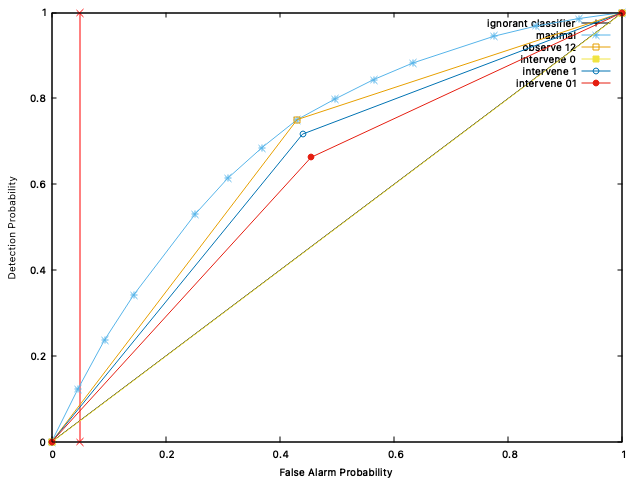
\includegraphics[width=0.85\linewidth]{example_operational_characteristic.png}

This shows the $(P_f, P_d)$ characteristic for varying $\eta$ for various experiments. Further details to be expounded upon soon.


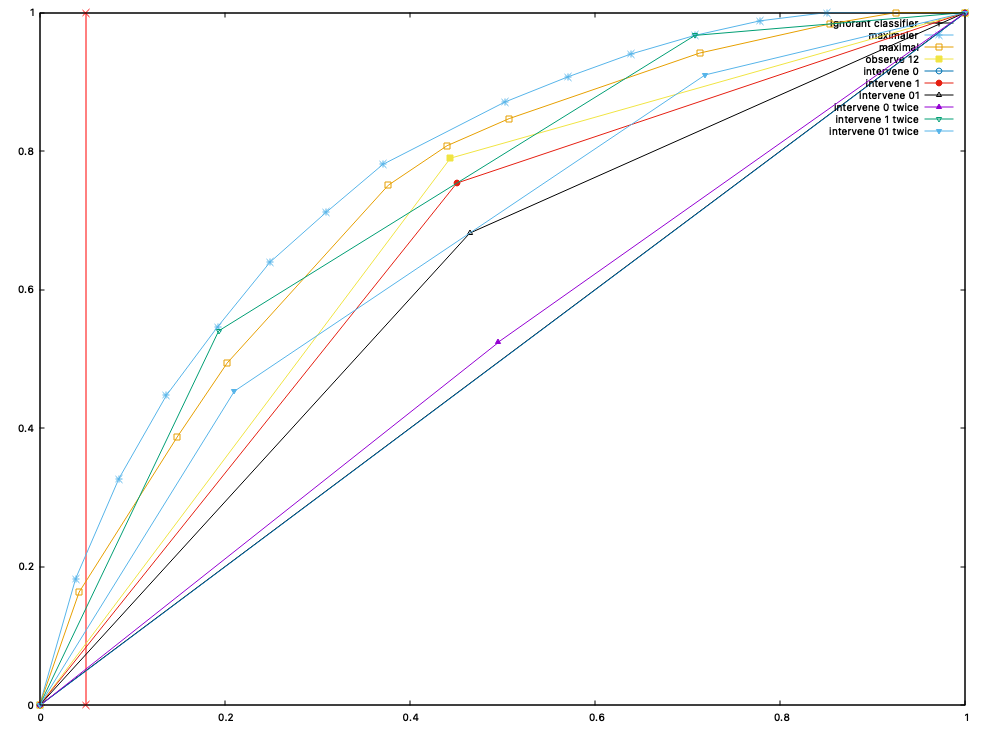
\includegraphics[width=0.85\linewidth]{bigger_pic.png}

This shows the frontiers for a wider range of programs, whose definitions in our ocaml version of this math is also provided below (for loose reference). In particular, this latter graph shows that not all estimators exhibit uniform prefernetiablity.

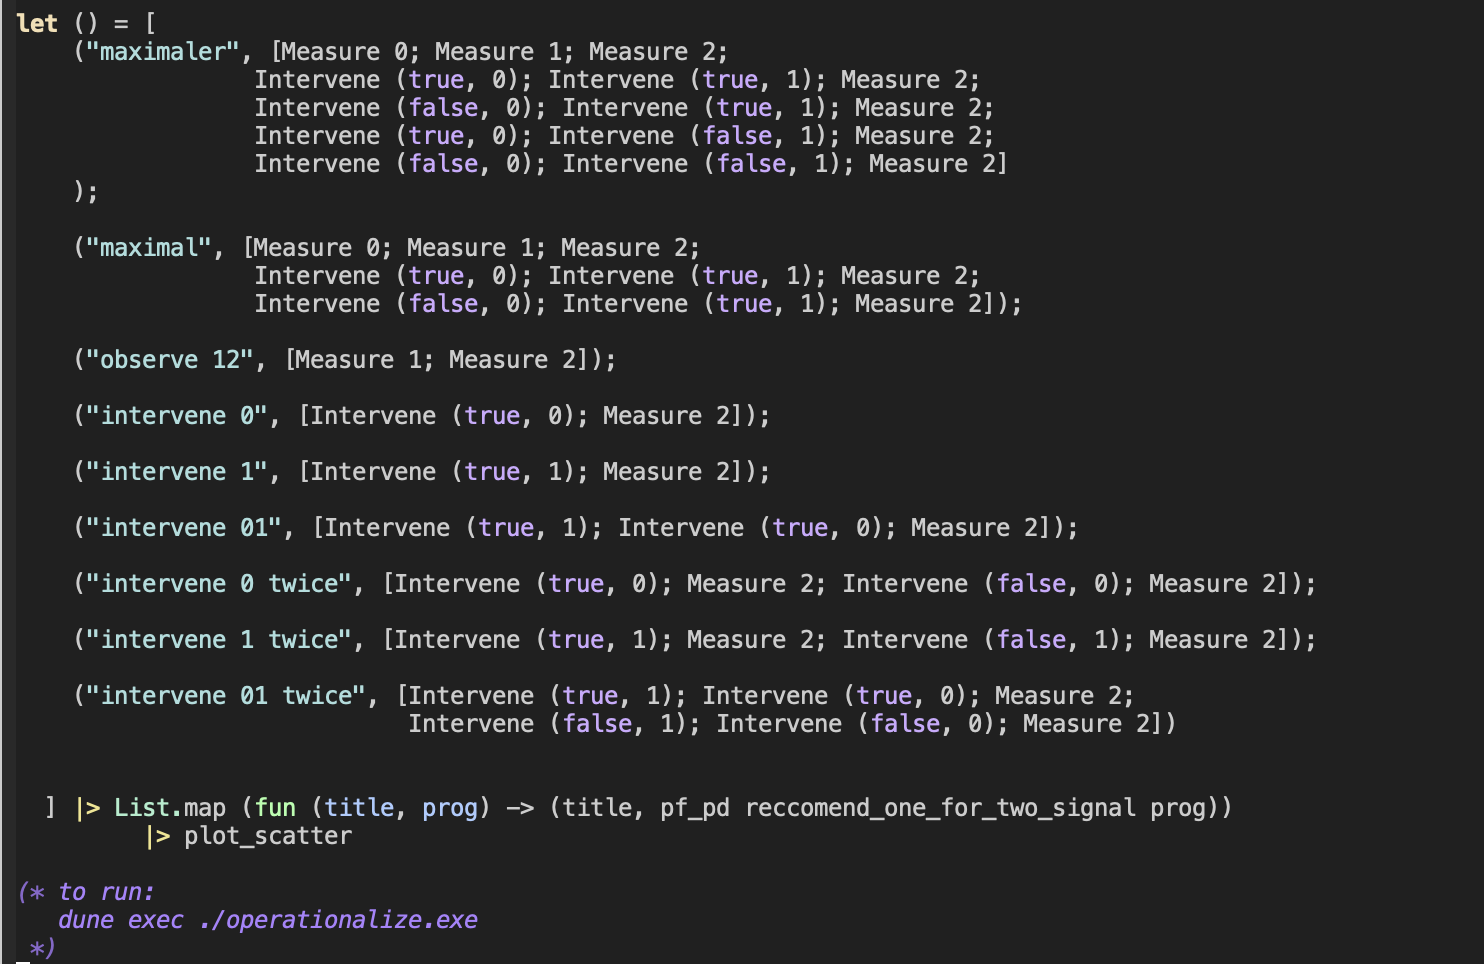
\includegraphics[width=0.85\linewidth]{code.png}

 \end{document}